%% ============================================================
%% LegalShadow — ICI2ST 2026 · CONFERENCE VERSION ·  Proceeding Paper
%% ------------------------------------------------------------
%% REV1 — revisión editorial aplicada (9 ago 2026)
%% Todos los cambios llevan un comentario "% REV1:" en la línea previa.
%% Los puntos que requieren confirmación del autor llevan "% AUTOR:".
%% Correcciones aplicadas:
%%   H-1  Figura 2b: se añade la dimensión Security; encendido PARCIAL
%%        (raíz vs. subconceptos) coherente con la Tabla 1.
%%   H-2  S_d unificado entre Fig. 1 y Fig. 2b; caption marcado "schematic".
%%   H-3  Barrido de sensibilidad desambiguado (SDS_global vs. Psi_global).
%%   H-4  \dataavailability sin "on request"; DOI Zenodo + hash del ledger.
%%   H-5  4 dimensiones declarativas vs. 10 ontológicas, declarado explícito.
%%   H-6  Fila global de la Tabla 1 re-rotulada + nota de agregación.
%%   H-7  Redondeos: Psi a 3 decimales; 48.2 / 90.4 % / 7.1 recalculados.
%%   H-8  17 corridas / 5 regeneraciones / 37 entradas: definiciones aclaradas.
%%   H-9  Estabilidad de Psi_global reportada.
%%   H-10 Control sintético reformulado como control positivo.
%%   H-11 "tier" (LegalShadow) vs. "layer" (ecosistema observado).
%%   H-12 Título: "Judicial Digital Ecosystems".
%%   m-1..m-12 Estilo, gramática, ortografía británica, robots.txt, keywords,
%%        pregunta de investigación, hallazgo reflexivo en el abstract.
%% ============================================================
\documentclass[engproc,proceedingpaper,submit,moreauthors]{Definitions/mdpi}
\usepackage{tikz}
\usetikzlibrary{arrows.meta,positioning,calc}
\usepackage{pgfplots}
\pgfplotsset{compat=1.17}
\usepackage{xcolor}
\newcounter{algo}
\renewcommand{\thealgo}{\arabic{algo}}

%% ── Colour palette (conceptual diagrams only; shadow data stays grey) ──
\definecolor{lsBlue}{HTML}{2563EB}
\definecolor{lsCyan}{HTML}{0891B2}
\definecolor{lsViolet}{HTML}{7C3AED}
\definecolor{lsAmber}{HTML}{D97706}
\definecolor{lsSlate}{HTML}{475569}

% REV1 (H-1): macro para dibujar una constelación con encendido parcial.
% #1 = ángulo polar · #2 = estilo del nodo raíz · #3 = lista offset/estilo
\newcommand{\lsconst}[3]{%
  \begin{scope}[shift={(#1:2.06)}]
    \node[#2] at (0,0.25) {};
    \foreach \o/\s in {#3}{\node[\s] at ({\o*0.17},-0.09) {};}
  \end{scope}}

%% MDPI internal commands
\firstpage{1}
\makeatletter
\setcounter{page}{\@firstpage}
\makeatother
\pubvolume{1}
\issuenum{1}
\articlenumber{0}
\pubyear{2026}
\copyrightyear{2026}
\datereceived{ }
\daterevised{ }
\dateaccepted{ }
\datepublished{ }
\doinum{}

\makeatletter
\renewcommand{\@doinum}{}
\makeatother

% REV1 (H-12): el estudio observa el ecosistema digital público de una
% institución judicial; "LegalTech" es una de las diez dimensiones, no el objeto.
% AUTOR: si el comité prefiere conservar "LegalTech Ecosystems", revertir aquí
% y añadir en §1 una definición explícita que abarque el caso judicial público.
\Title{ LegalShadow: An Ontology-Guided Digital Shadow Architecture
        for Semantic Validation of Judicial Digital Ecosystems}

\newcommand{\orcidauthorA}{0000-0001-6285-7390} % P.M. Paccha-Angamarca
\newcommand{\orcidauthorB}{0000-0003-2916-0369} % E.J. Sacoto-Cabrera
\newcommand{\orcidauthorC}{0000-0002-7335-2571} % V.V. Velepucha-Bonett

\Author{
    Patricio M. Paccha-Angamarca $^{1,2,}$*\orcidA{},
    Erwin J. Sacoto-Cabrera $^{2}$\orcidB{} and
    V\'ictor V. Velepucha-Bonett $^{1}$\orcidC{}
}
\AuthorNames{
    Patricio M. Paccha-Angamarca,
    Erwin J. Sacoto-Cabrera and
    V\'ictor V. Velepucha-Bonett
}
\address{
    $^{1}$ \quad Software Engineering Creation, Application and Management Group (GI-CreAGSoft),
    National Polytechnic School, Ladr\'on de Guevara E11-253, Quito 170525, Ecuador;
    victor.velepucha@epn.edu.ec\\
    $^{2}$ \quad Cloud Computing, Smart Cities \& High-Performance Computing Group (GIHP4C),
    Salesian Polytechnic University, Calle Vieja 12-30, Cuenca 010105, Ecuador;
    esacoto@ups.edu.ec
}
\corres{Correspondence: patricio.paccha@epn.edu.ec}

% REV1 (H-5, H-7, m-7): se declara "four-dimension" vs. "ten-dimension",
% se corrige el control a 90.4 % y se añade el hallazgo reflexivo.
\abstract{
    Judicial digital transformation produces heterogeneous ecosystems whose governance maturity is rarely auditable in an automated, reproducible and semantically grounded way. We present \emph{LegalShadow}, an ontology-guided digital shadow architecture that builds a JSON-LD structural representation of a judicial institution's public digital ecosystem from read-only web evidence and validates it against a ten-dimension governance ontology (TOGAF, COBIT, ITIL, NIST CSF, artificial intelligence, distributed ledger technology, open data, security, interoperability and a LegalTech domain). A hierarchical coverage function \texorpdfstring{$\Psi$}{Psi} measures how much of each ontological dimension the shadow materialises, and a gap function \texorpdfstring{$\delta$}{delta} orders remediation. A containerised implementation was exercised on the Ecuadorian Judiciary Council over 17 dated runs (2 July--4 August 2026; 187 read-only requests, 170 snapshots re-verified by SHA-256 with 0 mismatches). The shadow (34 components, 32 flows, 7 ecosystem layers) yields a \emph{four-dimension} declarative maturity index of 46/100 (Level 3), yet \emph{ten-dimension} semantic coverage reaches only \texorpdfstring{$\Psi_{\mathrm{global}}=34.9\%$}{Psi_global=34.9\%}, against 90.4\% for a synthetic positive control; three dimensions have zero coverage. The finding is reflexive as well as diagnostic: the observed institution lacks the very instrument---embedded structured data and a documented public API---that the shadow needs in order to represent it. The distance between declared digitalisation and machine-actionable governance is the central result.
}
% REV1 (m-6): se añaden descriptores de indexación.
\keyword{
    digital shadow; ontology; semantic validation; JSON-LD; LegalTech; e-justice; e-government; open judicial data; digital maturity
}
\begin{document}
\section{Introduction}
\label{sec:intro}
    Judicial systems are digitalising rapidly, combining institutional portals, case management systems and statistical repositories into ecosystems where modern single-page applications, generic content managers and legacy applications coexist with uneven interoperability. E-justice research documents specific risk factors---organisational complexity, vendor dependence, fragmentation---that hinder governance \cite{Rosa2013}, while open government data studies report a persistent gap between nominal publication and effective machine-readable reuse \cite{Janssen2012,Attard2015}.

    % REV1 (m-11): párrafo reescrito para que la línea previa quede situada
    % entre trabajos de terceros y no lea como una continuidad cerrada.
    This investigation extends a prior line of work on judicial digital governance. A multidimensional architecture for LegalTech governance (MALTG) integrated enterprise standards with domain-specific technologies such as artificial intelligence and distributed ledgers \cite{paccha2026architecture}, in the tradition of integrative IT-governance frameworks \cite{DeHaes2013}; a subsequent structural digital twin operationalised that conceptualisation to assess governance conformance \cite{Paccha2026SDT}, yielding a formally validated ontology and reproducible software artefacts deposited in an open repository \cite{paccha2026zenodo}. Those works, however, validated \emph{internal} structural consistency against baseline configurations in controlled environments. The present study changes the object of measurement rather than refining the previous one: from a twin that simulates a system its authors configure, to a shadow that passively observes a public digital surface they do not control and cannot instrument.

    Cyber-physical systems engineering offers a suitable abstraction. Kritzinger et al.\ distinguish digital model, digital shadow and digital twin by the automation of the information flow between object and virtual counterpart \cite{Kritzinger2018}: in the \emph{digital shadow} the real-to-virtual flow is automatic while feedback stays under human control. This is exactly the right configuration for the judicial domain, where acting on public institutional infrastructure is a state competence and automatic intervention would be improper; the artefact's value lies in observation and diagnosis. The paradigm has expanded from manufacturing \cite{Tao2019} to cities and public services \cite{Shahat2021,Brauner2022}, and Sepasgozar warns that conflating twin and shadow delays adoption \cite{Sepasgozar2021}. Crucially, the systematic review of Karabulut et al.\ finds no established method to \emph{verify} that a twin actually materialises its semantic model \cite{Karabulut2024}. The legal domain, in turn, has a mature tradition in knowledge representation \cite{Casanovas2016} and judicial decision prediction \cite{Medvedeva2020}, but both presuppose accessible structured data.

    % REV1 (m-1): se corrige "To the best of our systematic comparison…".
    To the best of our knowledge, and on the basis of a systematic comparison of the works reviewed above, no reported architecture simultaneously (i) builds a structural digital shadow of a judicial technological ecosystem automatically from public web evidence, (ii) serialises it as a JSON-LD knowledge graph anchored to a governance ontology, and (iii) validates that anchoring through a hierarchical coverage metric.

    % REV1 (m-8): pregunta de investigación explícita.
    This gap yields the question that organises the paper: \emph{to what extent does the publicly observable digital surface of a judicial institution materialise, in machine-processable form, the governance semantics prescribed by the very frameworks the institution declares?} Accordingly, this paper contributes: \textbf{(C1)} the LegalShadow reference architecture and its coverage/gap model $\langle\Psi,\delta\rangle$; \textbf{(C2)} an auditable, non-invasive acquisition protocol with per-snapshot cryptographic provenance, specified as an executable procedure (Algorithm~\ref{alg:sds}); and \textbf{(C3)} an empirical study of the Ecuadorian Judiciary Council over 17 dated runs that quantifies the distance between declared digitalisation and machine-actionable governance, with a synthetic positive control isolating instrument effects from ecosystem effects.

%% ============================================================
\section{Formal Model}
\label{sec:formal}

The model answers one question with arithmetic instead of opinion: \emph{how much of what the governance standards prescribe can actually be seen in the institution's digital surface?} The ontology $\Omega=\langle C,P,I,\sigma\rangle$ states what should exist---classes $C$ carrying a maturity score $\sigma:C\to[0,100]$ assigned against the published rubric of Section~\ref{sec:results}; the shadow $\Delta=G(V,E,\lambda)$ records what was observed---components $V$, flows $E$, labels $\lambda$ carrying layer, evidence and metadata; and the anchoring $\Gamma:V\to 2^{C}$ links the two through the \texttt{maltg:mapsTo} property. The measurement then reduces to three steps.

\textbf{Step 1---what did we actually see?} Each component declares which ontology classes it materialises, so the classes evidenced anywhere in the ecosystem are the union of those declarations:
\begin{equation}
R \;=\; \bigcup_{v \in V} \Gamma(v) \;\subseteq\; C .
\label{eq:coverage-set}
\end{equation}

\textbf{Step 2---how much of a dimension is there?} A governance dimension $d$ is not a flat list: it has a \emph{root} concept $r_d$ (the framework itself, e.g.\ \texttt{ITIL}) and \emph{subconcepts} $S_d$ that make it concrete (e.g.\ incident management). Naming a framework without operationalising it differs from the converse, so the two parts are scored separately and added:
\begin{equation}
\Psi(d) \;=\; \underbrace{w_r \cdot \mathbb{1}\!\left[\, r_d \in R \,\right]}_{\text{is the framework there at all?}} \;+\; \underbrace{w_s \cdot \frac{\lvert S_d \cap R \rvert}{\lvert S_d \rvert}}_{\text{how much of its detail is there?}}\;\in\;[0,1],
\label{eq:psi}
\end{equation}
% REV1 (H-3): se desambigua la escala del barrido de sensibilidad.
with $w_r+w_s=1$. In plain terms, with the default $(w_r,w_s)=(0.40,\,0.60)$: \emph{40\% for showing up, 60\% for the substance}. Two consequences matter. Publishing more evidence can never lower the score, since both terms grow with $R$; and $\Psi(d)=1$ requires root \emph{and} every subconcept, so a perfect score is unreachable by declaration alone. The weights admit calibration by the analytic hierarchy process \cite{Saaty1990}---not performed here---and the conclusions do not depend on them: for the case of Section~\ref{sec:results}, sweeping $w_r$ over $[0.10,0.90]$ moves $\mathrm{SDS}_{\mathrm{global}}$ only from 26.9 to 23.9 (equivalently, $\Psi_{\mathrm{global}}$ from 36.4\% to 32.3\%) and leaves the top of the remediation agenda unchanged.

\textbf{Step 3---what is that worth, and what should be fixed first?} With $\mathrm{onto}(d)$ the maturity the ontology prescribes (the mean expert score of its classes), what the shadow delivers is that prescription discounted by visibility, and the gap is the remainder:
\begin{equation}
\mathrm{sds}(d) \;=\; \mathrm{onto}(d)\cdot\Psi(d),
\qquad
\delta(d) \;=\; \mathrm{onto}(d)\,\bigl(1-\Psi(d)\bigr).
\label{eq:delta}
\end{equation}
A dimension becomes a priority only when it is \emph{both} important (high $\mathrm{onto}$) \emph{and} poorly evidenced (low $\Psi$), so sorting by $\delta$ yields the remediation agenda directly. Aggregating with dimension weights $\omega_d$ summing to one---all equal here, since no expert panel was convened---gives the headline figure
\begin{equation}
\Psi_{\mathrm{global}}=\frac{\mathrm{SDS}_{\mathrm{global}}}{\mathrm{Onto}_{\mathrm{global}}}=\frac{\sum_d \omega_d\,\mathrm{sds}(d)}{\sum_d \omega_d\,\mathrm{onto}(d)}.
\label{eq:global}
\end{equation} The institutional index is read through a five-level step function $L$ (1~Initial 0--20, 2~In transition 21--40, 3~Defined 41--60, 4~Managed 61--80, 5~Optimised 81--100), analogous to IT governance maturity models \cite{DeHaes2013}. The \emph{coverage-scoring stage} is linear: computing $R$ costs $O(|V|\cdot k)$, with $k$ the mean number of anchors per component, and evaluating Equations~\eqref{eq:psi}--\eqref{eq:global} costs $O(\sum_d|S_d|)$. Ontology parsing and graph construction dominate the remaining cost and are performed once per ingestion; we therefore claim linearity for the scoring stage, not for the pipeline as a whole.

Figure~\ref{fig:psiexample} carries three real dimensions of the observed institution through the arithmetic, chosen because they exhibit the three qualitatively distinct outcomes. \emph{Open data} is fully covered ($\Psi=0.40\cdot 1+0.60\cdot\frac{4}{4}=1.00$). \emph{TOGAF} is partially covered: root absent, two of six subconcepts present ($\Psi=0.20$)---the institution exposes technology-architecture artefacts without an architecture practice around them. \emph{ITIL} is absent altogether ($\Psi=0$), losing all 79.5 points. A single scalar would report TOGAF and ITIL as ``both weak''; $\Psi$ distinguishes an incomplete practice from a missing one, and those call for different remediation.

\begin{figure}[H]
\centering
\begin{tikzpicture}[scale=1, transform shape,
  root/.style={draw, thick, rounded corners=3pt, minimum width=2.25cm, minimum height=0.58cm, font=\scriptsize, align=center},
  sub/.style={draw, rounded corners=2pt, minimum width=0.50cm, minimum height=0.40cm, font=\small},
  on/.style={fill=black!45, draw=black!70},
  off/.style={fill=white, draw=black!45, densely dashed},
  ttl/.style={font=\scriptsize\bfseries},
  res/.style={font=\scriptsize}]
\node[ttl] at (0,1.30) {Open data};
\node[root, on] at (0,0.72) {\texttt{OpenData\_Layer}};
\foreach \i in {0,1,2,3}{\node[sub, on] at ($(-0.84,0)+(\i*0.56,0)$) {};}
\node[res, align=center] at (0,-0.60) {$\Psi=0.40(1)+0.60\tfrac{4}{4}$\\[1pt] $=\mathbf{1.00}$ \quad $\delta=0.0$};

\node[ttl] at (4.6,1.30) {Governance (TOGAF)};
\node[root, off] at (4.6,0.72) {\texttt{TOGAF}};
\foreach \i/\s in {0/on,1/on,2/off,3/off,4/off,5/off}{\node[sub, \s] at ($(3.20,0)+(\i*0.56,0)$) {};}
\node[res, align=center] at (4.6,-0.60) {$\Psi=0.40(0)+0.60\tfrac{2}{6}$\\[1pt] $=\mathbf{0.20}$ \quad $\delta=48.2$};

\node[ttl] at (9.2,1.30) {Service mgmt (ITIL)};
\node[root, off] at (9.2,0.72) {\texttt{ITIL}};
\foreach \i in {0,1,2,3,4}{\node[sub, off] at ($(8.08,0)+(\i*0.56,0)$) {};}
\node[res, align=center] at (9.2,-0.60) {$\Psi=0.40(0)+0.60\tfrac{0}{5}$\\[1pt] $=\mathbf{0.00}$ \quad $\delta=79.5$};

\node[font=\small] at (4.6,-1.8) {%
  \tikz\node[sub,on]{};~evidenced in $R$ (lit) \quad
  \tikz\node[sub,off]{};~not evidenced (dim) \quad
};
\node[font=\small] at (4.6,-2.4) {%
  upper box $=$ root $r_d$; lower row $=$ subconcepts $S_d$};
\end{tikzpicture}
\caption{The coverage function on three real dimensions. Filled nodes are concepts evidenced by at least one shadow component; hollow dashed nodes are prescribed but unobserved. The subconcept counts shown here ($|S_d|=4$, $6$ and $5$) are the ontology's actual counts for these dimensions.\label{fig:psiexample}}
\end{figure}

% REV1 (m-2, H-6): se sustituye el resumen promocional por las dos propiedades
% del agregado que el lector necesita antes de la sección empírica.
Two properties of the aggregate deserve emphasis before the empirical section. First, $\Psi_{\mathrm{global}}$ is an $\mathrm{onto}$-weighted mean of the per-dimension coverages, not their unweighted mean: dimensions the ontology deems more mature carry proportionally more influence, so the same shortfall costs more in a high-$\mathrm{onto}$ dimension than in a low one. Second, every quantity in the model is a deterministic function of the ontology and of the evidence actually retrieved; no step involves a judgement made after the data were seen. The whole apparatus is therefore recomputable by a third party from the published rubric and the dated artefacts, which is what makes it an audit instrument rather than a scoring opinion.

%% ============================================================
\section{Architecture and Acquisition}
\label{sec:arch}

% REV1 (H-11): "tier" para LegalShadow, "layer" para el ecosistema observado.
% REV1 (m-3): el texto sobre modularidad se traslada aquí, donde corresponde.
LegalShadow is organised in four decoupled \emph{tiers} deployed as Docker containers: \textbf{acquisition}, which runs the web observation protocol; \textbf{semantic}, holding $\Omega$ in OWL~2 and producing $\Delta$ in JSON-LD; \textbf{validation}, computing $\Psi$, $\delta$ and $L$; and \textbf{presentation}, exposing a REST API and an interactive three-dimensional graph. Throughout the paper \emph{tier} denotes a component of LegalShadow itself, while \emph{layer} is reserved for the architectural layers of the observed ecosystem. Encapsulating each stage in its own container is not merely deployment convenience: it guarantees that evidence harvesting, knowledge-graph projection and metric evaluation cannot contaminate one another, so a defect in scoring can never alter the evidence it scores. The flow is unidirectional from the observed ecosystem to presentation---the architectural translation of the artefact's \emph{shadow} rather than twin character \cite{Kritzinger2018,Sepasgozar2021}. The evaluation cycle follows the MAPE-K loop of autonomic computing \cite{Kephart2003}, with the deliberate caveat that execution is restricted to recommendations: closing the loop on the observed system is the institution's prerogative.

    \textbf{Acquisition protocol.}
    % REV1 (m-5): se explicita el cumplimiento de robots.txt y la serialización
    % de peticiones, que es la primera objeción de un revisor de ética de scraping.
    % AUTOR: confirmar la redacción exacta contra la implementación.
    The tier issues read-only HTTP probes against public targets declared in a versioned seed file. Following the ethical and legal recommendations of the literature \cite{Krotov2020}, the agent identifies itself with an explicit \emph{User-Agent} stating its purpose, honours the target's \texttt{robots.txt} directives, accesses only unauthenticated public resources, submits no forms and performs no writes, keeps at most one request in flight per target, caps each response at 400~KB with a 10--12~s timeout, and records every capture with a UTC timestamp and SHA-256 checksum. Runs, verifications and methodological decisions are written to an append-only hash-chained ledger, so a third party can re-execute the capture at a new cut-off date, verify that cited snapshots were not altered, and audit the chronology. Deterministic \emph{signals} are then computed from the markup: generating technology, legacy links (JSF/PHP), SPA confirmation, references to open data and integrity policies, and---crucially---presence of embedded structured data (JSON-LD/\texttt{schema.org} \cite{Guha2016}) and of a documented public API.

    \textbf{Semantic projection.}
    Signals are projected into a JSON-LD instance whose \texttt{@context} reuses standard vocabularies (Dublin Core, SKOS, Schema.org) and defines the \texttt{maltg:} namespace for governance terms. JSON-LD was chosen for its native fit with web development \cite{Guha2016}, its gateway status into linked data \cite{Bizer2009} and its alignment with FAIR interoperability \cite{Wilkinson2016}. Each component is serialised with its layer, evidence (URL, status, size, latency), findings, gaps and anchoring $\Gamma$, turning the shadow into a queryable knowledge subgraph \cite{Hogan2021}. Because the anchoring is expressed in the \texttt{maltg:} namespace, every macro-level index remains traceable back to the individual HTTP response that justifies it.

    \textbf{The GET-SDS console} (Figure~\ref{fig:getsds}) implements the acquisition experiment. It takes a configurable target URL, runs the protocol, and renders $\Omega$ as a three-dimensional star field where each class is a star and each governance cluster a named constellation. The field starts uniformly dim; the scan lights only classes for which evidence was found, making $\Gamma$ and the coverage set $R$ of Equation~\eqref{eq:coverage-set} directly observable. Because the target URL is a parameter rather than a constant, the same console runs unchanged on any institution.

\begin{figure}[H]
\centering
% REV1 (H-1, H-2): estilos raíz/subconcepto elevados al nivel de la figura
% para que la leyenda pueda reutilizarlos.
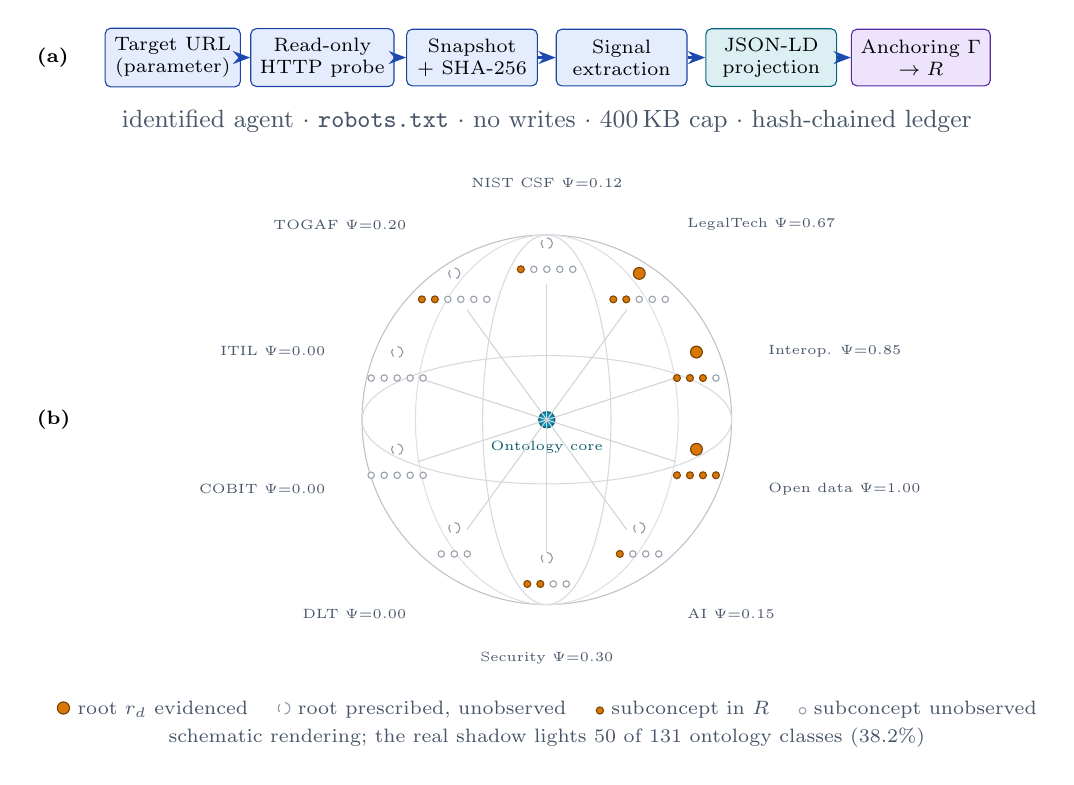
\begin{tikzpicture}[scale=1, transform shape,
  stg/.style={draw=lsBlue!70!black, rounded corners=2pt, minimum width=1.66cm, minimum height=0.72cm, align=center, font=\scriptsize, fill=lsBlue!12},
  arr/.style={-{Stealth[length=2.2mm]}, thick, lsBlue!75!black},
  rlit/.style={circle, fill=lsAmber, draw=lsAmber!55!black, inner sep=0pt, minimum size=4.4pt},
  rdim/.style={circle, fill=white, draw=lsSlate!60, densely dashed, inner sep=0pt, minimum size=4.2pt},
  slit/.style={circle, fill=lsAmber, draw=lsAmber!60!black, inner sep=0pt, minimum size=2.6pt},
  sdim/.style={circle, fill=white, draw=lsSlate!55, inner sep=0pt, minimum size=2.4pt},
  cst/.style={font=\tiny, text=lsSlate}]
\node[stg] (s0) at (0,0)    {Target URL\\\scriptsize(parameter)};
\node[stg] (s1) at (1.90,0) {Read-only\\HTTP probe};
\node[stg] (s2) at (3.80,0) {Snapshot\\+ SHA-256};
\node[stg] (s3) at (5.70,0) {Signal\\extraction};
\node[stg, draw=lsCyan!70!black, fill=lsCyan!14] (s4) at (7.60,0) {JSON-LD\\projection};
\node[stg, draw=lsViolet!70!black, fill=lsViolet!14] (s5) at (9.50,0) {Anchoring $\Gamma$\\$\rightarrow R$};
\foreach \a/\b in {s0/s1,s1/s2,s2/s3,s3/s4,s4/s5}{\draw[arr] (\a) -- (\b);}
\node[font=\small, text=lsSlate, anchor=north] at (4.75,-0.55)
  {identified agent $\cdot$ \texttt{robots.txt} $\cdot$ no writes $\cdot$ 400\,KB cap $\cdot$ hash-chained ledger};
\node[font=\scriptsize\bfseries, anchor=west] at (-1.85,0) {(\textbf{a})};

% ── (b) Esfera celeste: diez constelaciones con encendido parcial ──
\begin{scope}[shift={(4.75,-4.60)}, scale=0.97]
\draw[lsSlate!35] (0,0) circle (2.42);
\draw[lsSlate!22] (0,0) ellipse (2.42 and 0.84);
\draw[lsSlate!22] (0,0) ellipse (0.84 and 2.42);
\draw[lsSlate!18] (0,0) ellipse (1.72 and 2.42);
\node[circle, fill=lsCyan, draw=lsCyan!60!black, inner sep=0pt, minimum size=6pt] at (0,0) {};
\node[font=\tiny, text=lsCyan!60!black, anchor=north] at (0,-0.16) {Ontology core};
\foreach \a in {90,54,18,-18,-54,-90,-126,-162,162,126}{\draw[lsSlate!25] (0,0) -- (\a:1.78);}

% root evidenced + all subconcepts:            Psi = 1.00
\lsconst{-18}{rlit}{-1.5/slit,-0.5/slit,0.5/slit,1.5/slit}
\node[cst, anchor=west] at (-18:2.92) {Open data $\Psi{=}1.00$};
% root evidenced + 3 of 4 subconcepts:         Psi = 0.85
\lsconst{18}{rlit}{-1.5/slit,-0.5/slit,0.5/slit,1.5/sdim}
\node[cst, anchor=west] at (18:2.92) {Interop. $\Psi{=}0.85$};
% root evidenced + part of subconcepts:        Psi = 0.67
\lsconst{54}{rlit}{-2/slit,-1/slit,0/sdim,1/sdim,2/sdim}
\node[cst, anchor=south west] at (54:2.92) {LegalTech $\Psi{=}0.67$};
% root absent, 1 of 5 subconcepts:             Psi = 0.12
\lsconst{90}{rdim}{-2/slit,-1/sdim,0/sdim,1/sdim,2/sdim}
\node[cst, anchor=south] at (90:2.92) {NIST CSF $\Psi{=}0.12$};
% root absent, 2 of 6 subconcepts:             Psi = 0.20
\lsconst{126}{rdim}{-2.5/slit,-1.5/slit,-0.5/sdim,0.5/sdim,1.5/sdim,2.5/sdim}
\node[cst, anchor=south east] at (126:2.92) {TOGAF $\Psi{=}0.20$};
% root absent, no subconcepts:                 Psi = 0.00
\lsconst{162}{rdim}{-2/sdim,-1/sdim,0/sdim,1/sdim,2/sdim}
\node[cst, anchor=east] at (162:2.92) {ITIL $\Psi{=}0.00$};
\lsconst{-162}{rdim}{-2/sdim,-1/sdim,0/sdim,1/sdim,2/sdim}
\node[cst, anchor=east] at (-162:2.92) {COBIT $\Psi{=}0.00$};
\lsconst{-126}{rdim}{-1/sdim,0/sdim,1/sdim}
\node[cst, anchor=north east] at (-126:2.92) {DLT $\Psi{=}0.00$};
% root absent, 2 of 4 subconcepts:             Psi = 0.30
\lsconst{-90}{rdim}{-1.5/slit,-0.5/slit,0.5/sdim,1.5/sdim}
\node[cst, anchor=north] at (-90:2.92) {Security $\Psi{=}0.30$};
% root absent, 1 of 4 subconcepts:             Psi = 0.15
\lsconst{-54}{rdim}{-1.5/slit,-0.5/sdim,0.5/sdim,1.5/sdim}
\node[cst, anchor=north west] at (-54:2.92) {AI $\Psi{=}0.15$};
\end{scope}

\node[font=\scriptsize\bfseries, anchor=west] at (-1.85,-4.60) {(\textbf{b})};
\node[font=\scriptsize, text=lsSlate, anchor=north, align=center] at (4.75,-8.05)
  {\tikz\node[rlit]{};~root $r_d$ evidenced \quad \tikz\node[rdim]{};~root prescribed, unobserved \quad
   \tikz\node[slit]{};~subconcept in $R$ \quad \tikz\node[sdim]{};~subconcept unobserved\\[2pt]
   schematic rendering; the real shadow lights 50 of 131 ontology classes (38.2\%)};
\end{tikzpicture}
% REV1 (H-1): el caption ya no afirma un encendido binario.
\caption{The GET-SDS acquisition process. (\textbf{a}) Non-invasive pipeline, from a parameterised target URL to the coverage set $R$. (\textbf{b}) The ontology as a celestial sphere: each governance dimension is a constellation whose large marker is its root concept $r_d$ and whose small markers are its subconcepts $S_d$. Open data is fully lit; interoperability and the LegalTech domain are lit at the root and in part of their detail; TOGAF, NIST CSF, security and AI are lit \emph{only} at subconcept level, with no root---an incomplete practice; COBIT, ITIL and distributed ledger remain entirely dim---an absent one. The rendering is schematic: marker counts are illustrative rather than one-to-one with the 131 ontology classes.\label{fig:getsds}}
\end{figure}

Algorithm~\ref{alg:sds} states the procedure executed on every run, so that a third party can re-run it at a new cut-off date and compare artefacts.

\begin{figure}[H]
\centering
\begin{minipage}{\textwidth}
\small
\refstepcounter{algo}\label{alg:sds}%
\rule{\textwidth}{0.6pt}\\[2pt]
\textbf{Algorithm \thealgo:} Digital shadow generation and semantic validation\\[-6pt]
\rule{\textwidth}{0.4pt}
\begin{tabbing}
xx\=xx\=\kill
\textbf{Input:} seed targets $T$; ontology $\Omega$; dimensions $D$; weights $(w_r,w_s)$\\
\textbf{Output:} shadow $\Delta$; coverage set $R$; per-dimension $\Psi,\mathrm{sds},\delta$; index $L$\\[2pt]
1.\> \textbf{for each} $\tau\in T$: fetch $\tau$ read-only (identified agent, \texttt{robots.txt} honoured, 400\,KB cap);\\
\> store snapshot, record URL, UTC timestamp, bytes, latency and SHA-256 in the manifest\\
2.\> verify integrity: re-hash each snapshot, abort on mismatch, append the run to the ledger\\
3.\> extract deterministic signals from the markup (generator, legacy links, JSON-LD, API)\\
4.\> project signals into $\Delta=G(V,E,\lambda)$ and serialise as JSON-LD with the \texttt{@context} of $\Omega$\\
5.\> \textbf{for each} $v\in V$: resolve $\Gamma(v)\subseteq C$ via \texttt{maltg:mapsTo}; reject dangling identifiers\\
6.\> $R \leftarrow \bigcup_{v\in V}\Gamma(v)$\hfill\textit{// Eq.~\eqref{eq:coverage-set}}\\
7.\> \textbf{for each} $d\in D$: $\Psi(d)\leftarrow$ Eq.~\eqref{eq:psi}; then $\mathrm{sds}(d)$ and $\delta(d)$ by Eq.~\eqref{eq:delta}\\
8.\> aggregate to $\Psi_{\mathrm{global}}$ (Eq.~\eqref{eq:global}); $L\leftarrow$ band; sort $D$ by $\delta$ descending\\
9.\> persist the dated artefact with the ontology and shadow digests
\end{tabbing}
\vspace{-6pt}\rule{\textwidth}{0.6pt}
\end{minipage}
\end{figure}

%% ============================================================
\section{Case Study and Results}
\label{sec:results}

% REV1 (H-10): el control se presenta desde el inicio como control positivo.
The study applies LegalShadow to the public digital ecosystem of the Ecuadorian Judiciary Council (\texttt{funcionjudicial\-.gob\-.ec}) and validates the resulting shadow against the full ontology (131 classes, 144 relations, 14 cross-cutting), contrasted with a synthetic \emph{positive control}: a 39-component shadow authored to saturate the engine, whose role is to establish that the metric can approach unity on a well-anchored artefact.

\textbf{Scoring protocol.} The ontological scores $\sigma$ were not elicited ad hoc. Each of the ten dimensions has a versioned rubric fixing five observable levels (0, 25, 50, 75, 100) with explicit criteria---for TOGAF, for instance, level~50 requires the BDAT domains to be identified with named owners, and level~75 requires an operating ADM cycle with an architecture repository. A score with no associated evidence is flagged \emph{declared} rather than \emph{observed}, which is precisely what separates the declarative index of the next paragraph from the coverage figure that follows it. The rubric, the seed sources and the evidence manifests are versioned alongside the shadows, so the coding is auditable; it was, however, applied by the authors rather than by an independent panel (Section~\ref{sec:conclusions}).

% REV1 (H-8): las tres cardinalidades se definen para que no se confundan.
\textbf{Evidence corpus.} Over 17 dated runs between 2 July and 4 August 2026 the acquisition tier issued 187 read-only requests, of which 170 succeeded (90.9\%). Re-hashing every stored snapshot against its manifest yields \textbf{170 matches and 0 mismatches}: full integrity of the evidence base. The ledger holds 37 chained entries from \texttt{GENESIS} to head \texttt{6c7d2847932a606f}. Three cardinalities are reported in this section and they measure different things: a \emph{run} is one pass of the acquisition protocol; a \emph{shadow regeneration} is a run that additionally rebuilt $\Delta$ end to end, of which the series contains five; and a \emph{ledger entry} records a run, an integrity verification or a methodological decision, which is why the entries outnumber the runs. Latencies (median 788.5~ms, p95 954.4~ms, range 67--2810~ms) confirm the probe imposes negligible load, a design requirement of the ethical protocol \cite{Krotov2020}.

% REV1 (H-9): se reporta la estabilidad de Psi, no sólo la del índice declarativo.
% AUTOR: confirmar que Gamma (y por tanto R) fue idéntico en las cinco regeneraciones.
\textbf{Institutional shadow and declarative maturity.} The shadow from the 4 August run contains \textbf{34 components, 32 flows and 7 architectural layers} anchored to 11 seed sources, with anchoring \emph{total and referentially closed}: every component carries at least one anchor (mean 2.00, maximum 4) and all 50 distinct references resolve to existing ontology classes, with zero dangling identifiers. Signals show a modern portal on a generic content manager still surfacing 16 legacy links (6 JSF, 10 PHP), a confirmed case-consultation SPA with no documented public API, and the total absence of embedded JSON-LD despite declarative references to open data policies---exactly the gap between nominal publication and effective reuse reported in the open government literature \cite{Janssen2012,Attard2015}. The assessment over the four dimensions for which the institution publishes declarative evidence gives a global index of \textbf{46/100}, which $L$ places at Level 3 (``Defined''): data and semantic interoperability 28, integration architecture 42, declared transformation 55, regulatory compliance 58. Both this index and the coverage figures reported below were invariant across the five regenerated shadows: the only signal that drifted in the series was the legacy PHP count (13~$\rightarrow$~10 between 5 and 30 July), attributable to content editing on the observed portal, and that signal anchors no ontology class, so the coverage set $R$---and with it $\Psi_{\mathrm{global}}$---did not change.

% REV1 (H-7): 90.4 % y 7.1 recalculados sobre valores sin redondear.
% REV1 (H-10): alcance del control explicitado.
\textbf{Ten-dimension semantic validation.} Applying the engine of Section~\ref{sec:formal} to the same real shadow (Table~\ref{tab:validation}, Figure~\ref{fig:gaps}) gives $\Psi_{\mathrm{global}}=25.8/73.9=\mathbf{0.349}$: the shadow materialises only 34.9\% of the maturity the ontology prescribes, leaving an aggregate gap of 48.2 points (65.1\%). The positive control reaches $\Psi_{\mathrm{global}}=66.9/73.9=90.4\%$ with a residual gap of 7.1. This rules out a ceiling artefact in the scoring engine and shows that the low real coverage is a property of the observed ecosystem rather than of the instrument; it does not, on its own, establish construct validity, since the control was authored by the same team (Section~\ref{sec:conclusions}).

A result visible only through the shared apparatus is that both shadows light almost the same number of stars---50 of 131 for the real shadow against 51 for the control---yet their global coverage differs by a factor of 2.6. Coverage \emph{breadth} is not what $\Psi$ measures: \emph{which} concepts are anchored matters far more than how many. The control spreads its 51 anchors across all ten dimensions; the real ecosystem concentrates its 50 in open data, interoperability and LegalTech, leaving whole dimensions untouched. A naive count of evidenced nodes would have rated the two artefacts equivalent.

Three dimensions have \emph{zero} coverage because neither root nor subconcepts appear in $R$: service management (ITIL, $\delta=79.5$), control (COBIT, $\delta=62.7$) and distributed ledger ($\delta=52.4$). Four more are lit only below the root---AI, NIST CSF, security posture and TOGAF---which is a different condition and calls for different remediation. The single largest gap is AI integration ($\delta=82.4$), where a high ontological score (96.9) is almost entirely unrealised. Conversely open data attains full coverage and interoperability 0.85, reflecting genuine participation in the national open data catalogue.

% REV1 (H-5): se declara que los dos números no se calculan sobre el mismo conjunto.
This is the central contrast, and its terms must be stated precisely. The 46/100 aggregates the four dimensions on which the institution itself publishes declarative evidence; $\Psi_{\mathrm{global}}$ spans the ten dimensions the ontology prescribes. The two are therefore not two measurements of one quantity, and the comparison is not a difference of degree on a shared scale: it contrasts what an institution reports \emph{on its own terms} with what its digital surface exposes \emph{on the frameworks' terms}. Read that way the result is sharper, not weaker---an institution can only report progress on the dimensions it has chosen to instrument, and the six dimensions absent from its own assessment are precisely those where the ontology finds no machine-processable trace at all.

\begin{table}[H]
\small
% REV1 (H-6, H-7): fila global re-rotulada y nota de agregación añadida.
\caption{Hierarchical coverage validation of the real institutional shadow, $(w_r,w_s)=(0.40,\,0.60)$. The last column reports the synthetic positive control for the same dimension. Aggregates follow Equation~\eqref{eq:global} with equal $\omega_d$ and are computed on unrounded values; $\Psi_{\mathrm{global}}$ is thus an $\mathrm{onto}$-weighted mean of the $\Psi(d)$ column, whose unweighted mean is 0.329 (real) and 0.900 (control).\label{tab:validation}}
\begin{tabularx}{\textwidth}{Xcccccc}
\toprule
\textbf{Dimension} & $\mathbf{onto(d)}$ & \textbf{Root} & $\mathbf{\Psi(d)}$ & $\mathbf{sds(d)}$ & $\boldsymbol{\delta}\mathbf{(d)}$ & $\mathbf{\Psi}$ \textbf{ctrl}\\
\midrule
AI integration            & 96.9 & No  & 0.150 & 14.5 & \textbf{82.4} & 0.85\\
Service management (ITIL) & 79.5 & No  & 0.000 & 0.0  & \textbf{79.5} & 1.00\\
Resilience (NIST CSF)     & 72.0 & No  & 0.120 & 8.6  & 63.4 & 1.00\\
Control (COBIT)           & 62.7 & No  & 0.000 & 0.0  & 62.7 & 1.00\\
Security posture          & 80.4 & No  & 0.300 & 24.1 & 56.3 & 1.00\\
Distributed ledger        & 52.4 & No  & 0.000 & 0.0  & 52.4 & 0.85\\
Governance (TOGAF)        & 60.3 & No  & 0.200 & 12.1 & 48.2 & 0.70\\
LegalTech domain          & 75.5 & Yes & 0.673 & 50.8 & 24.7 & 0.60\\
Interoperability          & 81.2 & Yes & 0.850 & 69.0 & 12.2 & 1.00\\
Open data                 & 78.5 & Yes & 1.000 & 78.5 & 0.0  & 1.00\\
\midrule
\textbf{Global (Eq.~\eqref{eq:global}, $\mathrm{onto}$-weighted)} & \textbf{73.9} & 3/10 & \textbf{0.349} & \textbf{25.8} & \textbf{48.2} & \textbf{0.904}\\
\bottomrule
\end{tabularx}
\end{table}

\begin{figure}[H]
\centering
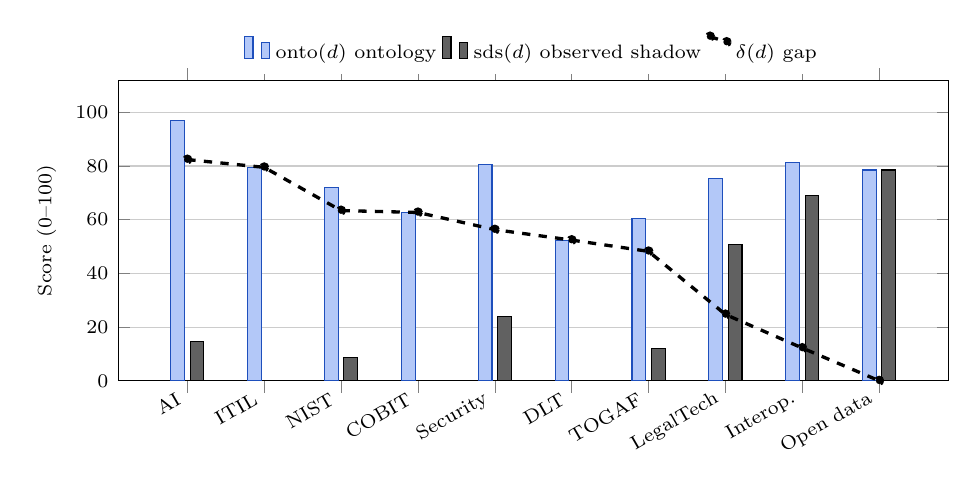
\begin{tikzpicture}
\begin{axis}[
  ybar,
  width=\textwidth, height=5.4cm,
  bar width=5pt,
  ymin=0, ymax=112,
  ylabel={Score (0--100)},
  ylabel style={font=\scriptsize},
  symbolic x coords={AI,ITIL,NIST,COBIT,Security,DLT,TOGAF,LegalTech,Interop.,Open data},
  xtick=data,
  x tick label style={rotate=30, anchor=east, font=\scriptsize},
  ytick={0,20,40,60,80,100},
  yticklabel style={font=\scriptsize},
  legend style={font=\scriptsize, at={(0.5,1.02)}, anchor=south, legend columns=3, draw=none},
  ymajorgrids, major grid style={black!20},
]
\addplot+[draw=lsBlue!80!black, fill=lsBlue!35] coordinates
  {(AI,96.9) (ITIL,79.5) (NIST,72.0) (COBIT,62.7) (Security,80.4) (DLT,52.4) (TOGAF,60.3) (LegalTech,75.5) (Interop.,81.2) (Open data,78.5)};
\addplot+[draw=black, fill=black!62] coordinates
  {(AI,14.5) (ITIL,0) (NIST,8.6) (COBIT,0) (Security,24.1) (DLT,0) (TOGAF,12.1) (LegalTech,50.8) (Interop.,69.0) (Open data,78.5)};
\addplot[sharp plot, very thick, dashed, black, mark=*, mark size=1.2pt] coordinates
  {(AI,82.4) (ITIL,79.5) (NIST,63.4) (COBIT,62.7) (Security,56.3) (DLT,52.4) (TOGAF,48.2) (LegalTech,24.7) (Interop.,12.2) (Open data,0)};
\legend{$\mathrm{onto}(d)$ ontology, $\mathrm{sds}(d)$ observed shadow, $\delta(d)$ gap}
\end{axis}
\end{tikzpicture}
\caption{Ontological versus effective maturity of the real institutional shadow, ordered by decreasing gap. The dashed line traces $\delta(d)$ and constitutes the remediation agenda.\label{fig:gaps}}
\end{figure}

%% ============================================================
\section{Discussion and Conclusions}
\label{sec:conclusions}

\textbf{Declarative maturity is not machine-actionable governance.} On the four dimensions it instruments itself, the institution scores 46/100, a figure a conventional assessment would report as reasonable progress. Evaluated against the semantics of the ten dimensions prescribed by the very frameworks it invokes, its observable ecosystem materialises 34.9\%, with three dimensions at zero anchored concepts and four more lit only below the root. The instrument separates what an institution \emph{declares} from what its digital surface \emph{exposes in machine-processable form}---quantities that maturity questionnaires conflate, and that differ not only in value but in the set of dimensions they can address at all.

\textbf{A reflexive finding.} The most deficient signal is precisely the absence of JSON-LD and of a public API: the observed institution lacks the very instrument---structured data---that the digital shadow uses to represent it. Adopting semantic markup would, besides improving findability \cite{Guha2016}, directly lift the weakest dimension and let third parties build value-added services on judicial data \cite{Attard2015,Wilkinson2016}.

\textbf{Contribution to an open problem.} Karabulut et al.\ note the absence of methods to verify that a twin materialises its semantic model \cite{Karabulut2024}. $\Psi$ offers an operational answer: computable in linear time, bounded, monotone, and interpretable dimension by dimension, it enables continuous audits of ontology--artefact alignment, and its root/subconcept decomposition localises the deficit---distinguishing ITIL (entirely absent) from TOGAF (an incomplete practice) and from interoperability (near-complete), distinctions no scalar score can express.

% REV1 (H-10): se añade la limitación de validez de constructo del control.
\textbf{Limitations.} The shadow observes only the \emph{public surface}: scores are \emph{observable} maturity, a lower bound on real maturity, and dimensions such as ITIL or COBIT may operate internally without public trace, so their zero coverage measures published evidence rather than practice. The ontological scores $\sigma$ were assigned by the authors against the versioned rubric rather than elicited from an independent panel; no Delphi round, content-validity ratio \cite{Lawshe1975} or inter-rater agreement has yet been computed, so $\mathrm{onto}(d)$---and therefore the absolute value of $\delta$---carries unquantified judgement. The synthetic control is a positive control only: authored by the same team to saturate the engine, it bounds instrument artefacts but does not establish construct validity, which would require an artefact whose true coverage is known independently. The sensitivity sweep bounds the effect of $(w_r,w_s)$ but not that of $\sigma$. Aggregation uses equal dimension weights. External validity is limited to one institution studied in depth over one month, so the reported stability of $\Psi_{\mathrm{global}}$ speaks to instrument repeatability, not to the ecosystem's behaviour over longer horizons. Signal detection depends on portal markup stability; the cryptographic record attenuates, without eliminating, observer drift.

% REV1 (m-10): se suaviza el claim de neutralidad geográfica, no demostrado.
\textbf{Conclusions and future work.} LegalShadow instantiates the digital shadow paradigm over a judicial technological ecosystem with three distinctive properties: automatic generation from public web evidence with cryptographically verifiable provenance, semantic grounding in a multi-standard governance ontology serialised in JSON-LD, and quantitative validation through $\Psi$ and $\delta$. Every figure reported here is recomputable by a third party from the published rubric and the dated artefacts, which is the property that turns the instrument into an audit rather than an assessment. Nothing in the architecture is country-specific \emph{by construction}---the ontology encodes international frameworks, the protocol runs over standard HTTP, the context reuses global vocabularies---though transferability remains to be demonstrated empirically; dated shadows per institution would then enable longitudinal and cross-sectional comparison, extending to justice the logic of comparable urban twins \cite{Shahat2021}. Future work targets multi-institutional studies with full $\Psi/\delta$ evaluation per institution, independent elicitation of $\sigma$ to remove the judgement now embedded in $\mathrm{onto}(d)$, assisted loop closure preserving human decision under MAPE-K \cite{Kephart2003}, automatic ontology alignment to enrich $\Gamma$ \cite{Hogan2021}, and a behavioural dimension built on procedural performance indicators \cite{Medvedeva2020}.

\vspace{6pt}

\authorcontributions{Conceptualisation, methodology, software, validation and writing---original draft, P.M.P.-A.; supervision, formal analysis and writing---review and editing, E.J.S.-C. and V.V.V.-B. All authors have read and agreed to the published version of the manuscript.}

\funding{This research received no external funding.}
% REV1 (H-4): se elimina "on request", que contradecía la tesis de auditabilidad;
% se añaden DOI y el hash de cabeza del ledger para que la evidencia sea verificable.
% AUTOR: sustituir el DOI de marcador por el definitivo antes del envío final.
\dataavailability{
    The LegalShadow source code, the OWL governance ontology, the dated JSON-LD shadows and the SHA-256 evidence manifests are openly available without restriction at Zenodo (DOI:~10.5281/zenodo.XXXXXXX) \cite{paccha2026zenodo} and at \texttt{https://github.com/patmic/ArchLab}. The evidence base reported here corresponds to ledger head \texttt{6c7d2847932a606f}; any third party can recompute that head from the published manifests and so verify that no cited snapshot was altered. Observed data originate exclusively from public resources of the Ecuadorian Judiciary Council.
    \\
    \textbf{The code and instructions to reproduce the setup are available at:}
    \begin{itemize}
        \item git clone https://github.com/patmic/ArchLab,
        \item docker compose up -d -{}-build
        \item and, access the dashboard at http://localhost:8080.
    \end{itemize}
}

\conflictsofinterest{The authors declare no conflicts of interest.}

%% ============================================================
\begin{adjustwidth}{-\extralength}{0cm}
\reftitle{References}
\bibliography{ICI2ST_LegalShadow_Ref}
\end{adjustwidth}

\end{document}
